\documentclass{article}
\usepackage{amsmath}
\usepackage{booktabs, graphicx, wrapfig}
\usepackage{geometry}
\geometry{margin=1in}
\usepackage{amsthm}
\usepackage{makecell}

\usepackage{listings}
\lstset{%
        language=python,
        keepspaces=false,
        basicstyle=\small\ttfamily,
       commentstyle=\footnotesize\itshape{},
       identifierstyle=\slshape{},
       keywordstyle=\bfseries,
       numbers=left,
       numberstyle=\tiny{},
       numberblanklines=false,
       inputencoding={utf8},
       columns=fullflexible,
       basewidth=.1em,
        fontadjust=true,
        tabsize=4,
        emptylines=*1,
       breaklines,
       breakindent=3pt,
        prebreak=\smash{\raisebox{-.5ex}{\hbox{\tiny$\hookleftarrow$}}},
    escapeinside={//*}{\^^M} % Allow to set labels and the like in comments starting with //*
	}

\newtheoremstyle{note}% <name>
{0pt}% <Space above>
{5pt}% <Space below>
{}% <Body font>
{}% <Indent amount>
{\itshape}% <Theorem head font>
{}% <Punctuation after theorem head>
{.1em}% <Space after theorem headi>
{}% <Theorem head spec (can be left empty, meaning `normal')>
\theoremstyle{note}
\newtheorem{definition}{Definition}[section]


\title{CS486 Summarize}
\author{}
\date{}

\begin{document}

\section{Agents and Abstraction}

\begin{definition}[Planning Horizon]:
\begin{itemize}
    \item \textbf{Static:} The world does not change over time.
    \item \textbf{Finite Horizon:} The agent reasons about a fixed finite number of time steps.
     (Agent know when it will end)
    \item \textbf{Indefinite Horizon:} The agent reasons about a finite but not predetermined number of time steps, such as until goal completion.
    (Agent know it will end, but not sure when)
    \item \textbf{Infinite Horizon:} The agent plans as if it will continue operating forever.
    (agent know it will never end)
\end{itemize}
\end{definition}

\begin{definition}[Representation]:
\begin{itemize}
    \item \textbf{Explicit States:} A state represents one possible configuration of the world.
    \item \textbf{Features:} Natural descriptors of states. (binary features can represent exponentially many states)
    \item \textbf{Individuals and Relations:} Use feature for reasoning about individuals and their relationships without necessarily knowing all individuals or when there are infinitely many individuals.
\end{itemize}
\end{definition}

\begin{definition}[Computational Limits]:
\begin{itemize}
    \item \textbf{Perfect Rationality:} The agent always selects the optimal action, which is often not possible in practice.
    \item \textbf{Bounded Rationality:} The agent selects a possibly sub-optimal action given its limited computational resources.
\end{itemize}
\end{definition}

\begin{definition}[Uncertainty]:
\begin{itemize}
    \item \textbf{fully observable:} agent knows the state of the world from the observation
    \item \textbf{partially observable:} there can be many state that are possible given an observation.
\end{itemize}
\end{definition}

\begin{definition}[Uncertain Dynamics]:
\begin{itemize}
    \item \textbf{Deterministic:} The outcome of an action is always the same.
    \item \textbf{Stochastic:} There is uncertainty over the states resulting from executing a given action.
\end{itemize}
\end{definition}

\begin{definition}[Goals or Complex Preferences]:
\begin{itemize}
    \item \textbf{Achievement Goals:} Goals that an agent aims to achieve, which can be represented as complex logical formulas.
    \item \textbf{Maintenance Goals:} Goals that an agent seeks to maintain over time.
    \item \textbf{Complex Preferences:} Involves trade-offs between various desiderata, potentially at different times, and may be either ordinal or cardinal (e.g: medical).
\end{itemize}
\end{definition}

\begin{definition}[Reasoning by Number of Agents]:
\begin{itemize}
    \item \textbf{Single Agent Reasoning:} The agent assumes any other agents are part of the environment, focusing on individual goal achievement.
    \item \textbf{Adversarial Reasoning:} The agent considers another agent acting in opposition to its goals, common in competitive settings.
    \item \textbf{Multi-agent Reasoning:} The agent strategically reasons about the actions and goals of other agents, which may be cooperative, competitive, or independent.
\end{itemize}
\end{definition}


%%%%%%%%%%%%%%

\section{Graph Search Algorithm}

% Table
\begin{table}[h!]
\begin{tabular}{@{}lllll@{}}
\toprule
\textbf{Algorithm} & \textbf{Frontier} & \textbf{Runtime} & \textbf{Space} & \textbf{halts?}\\ \midrule
\textbf{uninformed} (no heuristic)\\
Depth-First Search & LIFO & Exp / $O(b^m)$ & Linear / $O(bm)$ & No\\
Breadth-First Search & FIFO & Exp / $O(b^{d})$ & Exp / $O(b^{d})$ & Yes\\
Lowest-Cost-First Search & Lowest cost & Exp & Exp & Yes\\
Dijkstra's Algorithm* & Lowest cost & $O((V+E) \log V)$ & $O(V^2)$ \\
Iterative-Deepening Search* & LIFO in FIFO \textsuperscript{1} & Exp / $O(b^{d})$ & Linear / $O(bd)$ & Yes \textsuperscript{2}\\\\

\textbf{informed} (has heuristic)\\
(Greedy) Best-First Search & Global min heuristic & Exp & Exp & No \\
Heuristic Depth-First Search &  Local min heuristic (LIFO) &  Exp / $O(b^m)$ & Linear / $O(bm)$  & No\\
A* Search & Lowest (cost + heuristic) & Exp & Exp & Yes\\ \bottomrule
\end{tabular}
% description
\footnotesize{\\ $b$ is the branching factor \\ $m$ is the maximum depth of the search tree \\ $d$ is the depth of the shallowest goal node.}\\\\
\footnotesize{\textsuperscript{1} a BFS but for every depth limit do a DFS} \\
\footnotesize{\textsuperscript{2} Guaranteed to terminate at depth $d$}
%\caption{Comparison of Graph Search Algorithms}
\end{table}

% Table
\begin{table}[h!]
\begin{tabular}{@{}lll@{}}
\toprule
\textbf{Algorithm} & \textbf{Completeness} & \textbf{Optimality} \\ \midrule
\textbf{uninformed} (no heuristic)\\
Depth-First Search & No (fails for infinite cycle) & No (not considering all possibilities) \\
Breadth-First Search & Yes & Yes (if cost is uniform)\\
Lowest-Cost-First Search & Yes & Yes\\
Dijkstra's Algorithm* & Yes & Yes \\
Iterative-Deepening Search* & Yes (Same as BFS) & No (but guaranteed shallowest goal) \\\\

\textbf{informed} (has heuristic)\\
(Greedy) Best-First Search & No (fails for infinite cycle) & No (from not considering cost of arc)\\
Heuristic Depth-First Search & No (fails for infinite cycle) & No (not considering all possibilities)\\
A* Search & Yes\textsuperscript{1}  & Yes\textsuperscript{1} \\ \bottomrule
\end{tabular}\\
% description
\footnotesize{\textsuperscript{1} Assuming heuristic is \textbf{admissible}, branch factor is \textbf{finite}, and arc cost are bounded \textbf{above zero}} \\
\footnotesize{If \(h\) satisfies the \textbf{monotone restriction}, $A^*$ with \textbf{multiple path pruning} \textbf{always finds the shortest path} to a goal}.

%\caption{Completeness and Optimality of Graph Search Algorithms}
\end{table}



% Definitions
\begin{definition}[Admissible]
An \textbf{Admissible} heuristic \textbf{never overestimate} the cost from \textbf{any node to the goal}. An \textbf{Admissible} search algorithm returns an \textbf{optimal solution} if it exists.
\end{definition}

\begin{definition}[Monotone / Consistent]
A heuristic function \(h\) satisfies the \textbf{monotone restriction} if \textbf{$h(m) - h(n) \le \text{cost}(m,n) \text{ for every arc} <m,n>$}. (The heuristic of a path is always less than or equal to the true cost)
\end{definition}

\textbf{Monotonicity} is like \textbf{admissibility} but \underline{between any two nodes}.

So, a \textbf{consistent} heuristic is \textbf{admissible}, but a \textbf{admissible} heuristic is not necessarily \textbf{consistent}.

\newpage

\section{Adversarial Search(Minimax)}

\begin{itemize}

  \item 
  \begin{verbatim}
	function minimax (node, depth, maximizingPlayer) is
    if depth = 0 or node is a terminal node then
        return the heuristic value of node
    if maximizingPlayer then
        value := -inf
        for each child of node do
            value := max(value, minimax(child, depth - 1, FALSE))
        return value
    else (* minimizing player *)
        value := inf
        for each child of node do
            value := min(value, minimax(child, depth - 1, TRUE))
        return value
	\end{verbatim}
  \item \textbf{Suitable Type of Problem:}
  \begin{itemize}
    \item Competitive two-person, zero-sum games.
    \item Two players take turns to move and the one winner one loser.
  \end{itemize}

  \item \textbf{Idea:}
  \begin{itemize}
    \item Find \textbf{best option} for you on nodes you control (MAX)
    \item Assumes opponent will take \textbf{worst option} for you on their node (MIN)
    \item Recursively search leaf nodes and percolate optimal value upward
  \end{itemize}

  \item \textbf{Pruning Methods:}
  \begin{itemize}
    \item \textbf{Alpha-beta Pruning:}
    \begin{itemize}
      \item Ignore portions of the search tree without losing optimality
      \item doesn not change worst-case performance (Exp)
    \end{itemize}
    \item \textbf{Heuristic Pruning (Early Stopping):}
    \begin{itemize}
      \item Heuristics are used to evaluate the potential of non-terminal states.
      \item This method saves computational resources but may not always yield the optimal solution.
    \end{itemize}
  \end{itemize}
\end{itemize}


\section{Higher level strategies}
% Table
\begin{table}[h!]
\begin{tabular}{@{}llll@{}}
\toprule
\textbf{Search} &\textbf{\makecell[l]{Search\\ Complexity}} & \textbf{Difficulty} & \textbf{Reason to Win} \\ \midrule
\textbf{Symmetric } & $b^n$ & \makecell[l]{Not able to construct \\ backward on dynamically \\ constructed graph} & \makecell[l]{Choose between forward / backward\\search based on branching factor} \\ \midrule
\textbf{Bidirectional } & $2b^{\frac{k}{2}} << b^k$ & Make sure frontiers meet & \makecell[l]{Searches forward and backward \\simultaneously, leading to exponential \\savings in time and space.} \\ \midrule
\textbf{Island-Driven } & $mbk^{\frac{k}{m}} << b^k$ & \makecell[l]{identify islands \\ hard to guarantee optimality} & \makecell[l]{Decomposes the problem \\into $m$ smaller subproblems, \\each of which is easier to solve.} \\ \bottomrule
\end{tabular}
%\caption{Comparison of High-Level Search Strategies}

% description


\end{table}


%%%%%%%%%

\section{Constraint Satisfaction Problems (CSPs)}

\begin{itemize}
  \item \textbf{Definition:}
  \begin{itemize}
    \item Set of \textbf{variables},  \textbf{domain for each variable}, set of \textbf{constraints} or \textbf{evaluation function}.
    \item \textbf{Solution} is an assignment to the \textbf{variables} that satisfies \textbf{all constraints}.
    \item \textbf{Solution} is a \textbf{model of the constraints}.
  \end{itemize}

  \item \textbf{Problem Types:}
  \begin{itemize}
    \item \textbf{Satisfiability Problems:} Find assignment satisfies the given hard constraints.
    \item \textbf{Optimization Problems:} Find assignment optimizes the evaluation function(soft constraints).
  \end{itemize}

  \item \textbf{Search Representation:}
  
    % Table
	\begin{tabular}{@{}ll@{}}
	\toprule
 	\textbf{Assignment Type} & \textbf{Description} \\ \midrule
	Complete Assignment & \makecell[l]{Node is  assignment of value to all variables. \\Neighbours are created by changing one variable value.} \\ \midrule
	Partial Assignment & \makecell[l]{Nodes is assignment to the first \(k-1\) variables. \\Neighbours are formed by assigning a value to the \(k^{th}\) variable.} \\
	\bottomrule
	\end{tabular}
	%\caption{CSP Representations as Graph Searching Problems}


  \item \textbf{Dual Representations of Crossword Puzzle:}
  
  	% Table
	\begin{tabular}{@{}llll@{}}
	\toprule
 	\textbf{Type} & \textbf{Nodes} & \textbf{Domains} & \textbf{Constraints} \\ \midrule
	Primal & word positions & letters & intersecting letters are same \\ \midrule
	Dual & squares & letters & words must fit \\
	\bottomrule
	\end{tabular}

  \item \textbf{Example of CSP Setup:}
   
   % Table
   \begin{tabular}{@{}llll@{}}
   \toprule
   \textbf{Problem} & \textbf{Variables} & \textbf{Domains} & \textbf{Constraints} \\ \midrule
   Crosswords & letters & a-z & words in dictionary \\ \midrule
   Crosswords & words & dictionary & letters match \\ \midrule
   Scheduling & times & times,dates & before, after \\
 & events & types & same resource \\
 & resources & values & \\ \midrule
Party Planning & guests & values & cliques \\ \midrule
Ride Sharing & people/trips & locations & cars \\
\bottomrule
\end{tabular}

  \item \textbf{Constraints \& Solution}
  \begin{itemize}
    \item \textbf{Constraints}: Can be \textbf{N-ary} or \textbf{Binary}.
    \item \textbf{Solutions}:
    \subitem \textbf{Generate and Test} 
    
    Exhaustively check all combinations against constraints.
    \subitem \textbf{Backtracking} 
    
    Prune large portions of the state space by ordering variables and evaluating constraints.
    
    Efficiency depends on \textbf{order} of variables.
    
    Find optimal ordering is \textbf{as hard} as solving the problem.
    
    Cut off large branches as soon as possible, push failures as high as possible.
    
     
    \subitem \textbf{Consistency Techniques} 
    
    Look for inconsistencies to simplify the problem / Graphical representation
  \end{itemize}
  
  \item\textbf{Constraint Network (CN)}
  	
  	\begin{itemize}
    \item \textbf{Domain constraint}: 
    
    unary constraint of values $x$ on values in a domain, $<X,c(X)>$
    \item \textbf{Domain consistent}: 
    \subitem A \textbf{node} is \textbf{Domain consistent} if no domain value violates any domain constraints. 
    \subitem A \textbf{CN} is \textbf{Domain consistent} if all nodes are \textbf{Domain consistent}.
    
    \item \textbf{Arc} $<X, c(X,Y)>$ is:
    \subitem A \textbf{constraint} on $X$ posed by $Y$.
    \subitem  \textbf{Arc consistent} if for all $X \in D_X$, there exist some $Y \in D_Y$ such that $c(X,Y)$ is satisfied.
    
  	\item \textbf{CN} is \textbf{Arc consistent} if all arcs are \textbf{arc consistent}.
  	
  	\item set of variables $\{X_1,X_2, \dots, X_N\}$ is \textbf{path consistent} if all \textbf{arcs} and \textbf{domains} are \textbf{consistent}

  \end{itemize}
  	% figure of CSP
  	\begin{figure*}[!htbp]
  	\center
  	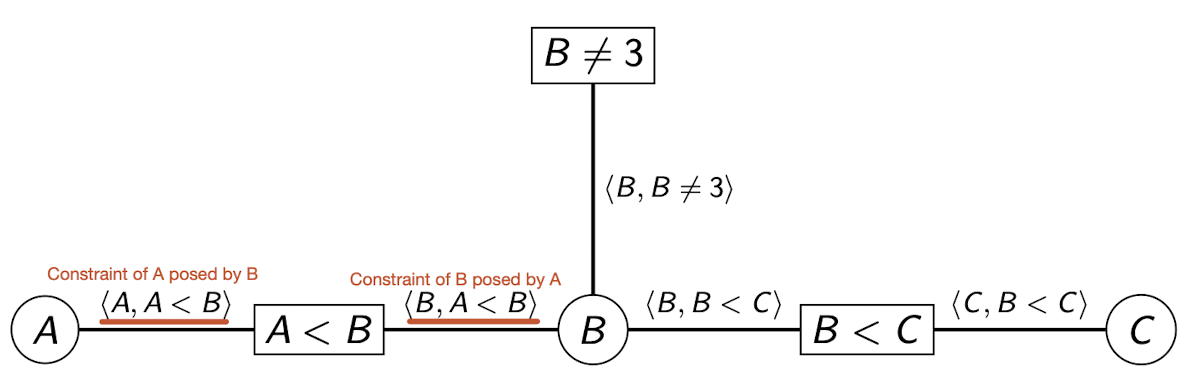
\includegraphics[width=7cm]{CSP_Graph.png}
  	\end{figure*}
  	
  	%%%%%%%%%% AC-3
  \item\textbf{AC-3 (CN) algorithm} (Alan Mackworth, 1977)
  
  \begin{itemize}
  \item \textbf{Purpose:} Makes a Constraint Network (CN) arc consistent and domain consistent.
  \item \textbf{Procedure:}
  \begin{itemize}
    \item Initialize the To-Do Arcs Queue (TDA) with all inconsistent arcs.
    \item Make all domains domain consistent.
    \item Put all arcs in TDA.
    \item Repeat until TDA is empty:
    \begin{itemize}
      \item Select and remove an arc $<X, c(X,Y)>$ from TDA.
      \item Remove all values from the domain of X that:
      \subitem do not have a corresponding value in the domain of Y 
      \subitem satisfying the constraint $c(X,Y)$.
      \item If any values were removed, for all $Z \neq Y$, add back arcs $<Z, c'(Z,X)>$ into TDA .
       (Add back all constraints posed to other variable by $X$. As the $X$ value enforced by the constraints / arc we removed is used by some other constraints posted by $X$ to other variables)
    \end{itemize}
  \end{itemize}
  \item \textbf{Termination:}
  \begin{itemize}
    \item AC-3 always terminates under one of three conditions:
    \begin{itemize}
      \item \textbf{Every domain is empty}: no solution.
      \item \textbf{Every domain has a single value}: a solution.
      \item \textbf{Some domains have 1+ value}: not sure if a solution exists.
      
      (further splitting and recursive call needed)
    \end{itemize}
  \end{itemize}
  \item \textbf{Properties:}
  \begin{itemize}
    \item Termination is guaranteed.
    \item Time complexity is $O(cd^3)$.\footnote{where $n$ is the number of variables, $c$ is the number of binary constraints, and $d$ is the maximum size of any domain}
    \item Consistency of each arc can be checked in \( O(d^2) \) time.
  \end{itemize}
  \item \textbf{Different elimination ordering} can result in \textbf{different size} of intermediate constraints.
  
  \item \textbf{Variable Elimination}
  \begin{itemize}
  \item \textbf{Concept:}
  \begin{itemize}
    \item Variables are eliminated one by one, transferring their constraints to neighbours.
    \item A single remaining variable with no values indicates an \textbf{inconsistent} network.
  \end{itemize}

  \item \textbf{Algorithm:}
  \begin{itemize}
    \item If only one variable remains, return the intersection of the unary constraints involving it.
    \item Select a variable \( X \).
    \subitem Join the constraints where \( X \) appears to form a new constraint \( R \).
    \subitem Project \( R \) onto other variables to form \( R_2 \).
    \subitem Place new constraint \( R_2 \) between all variables previously connected to \( X \).
    \subitem Remove \( X \) from the problem.
    \subitem Recursively solve the simplified problem.
    \subitem Return \( R \) joined with the solution from the recursive call.
  \end{itemize}

  \item Finding the optimal elimination ordering is as complex as the CSP itself.
\end{itemize}
	% figure of CSP
  	\begin{figure*}[!htbp]
  	\center
  	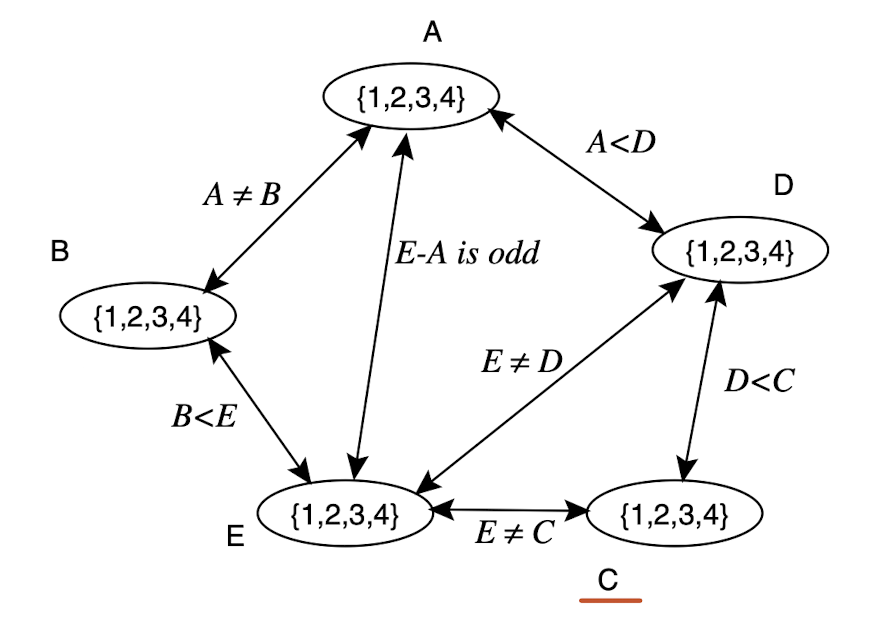
\includegraphics[width=5.5cm]{Variable_Elimination_1.png}
  	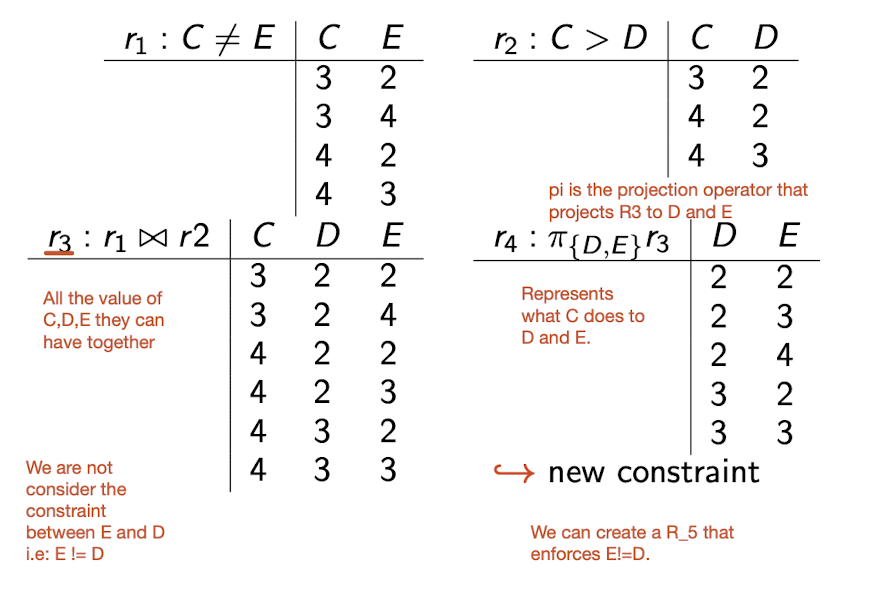
\includegraphics[width=5.5cm]{Variable_Elimination_3.png}
  	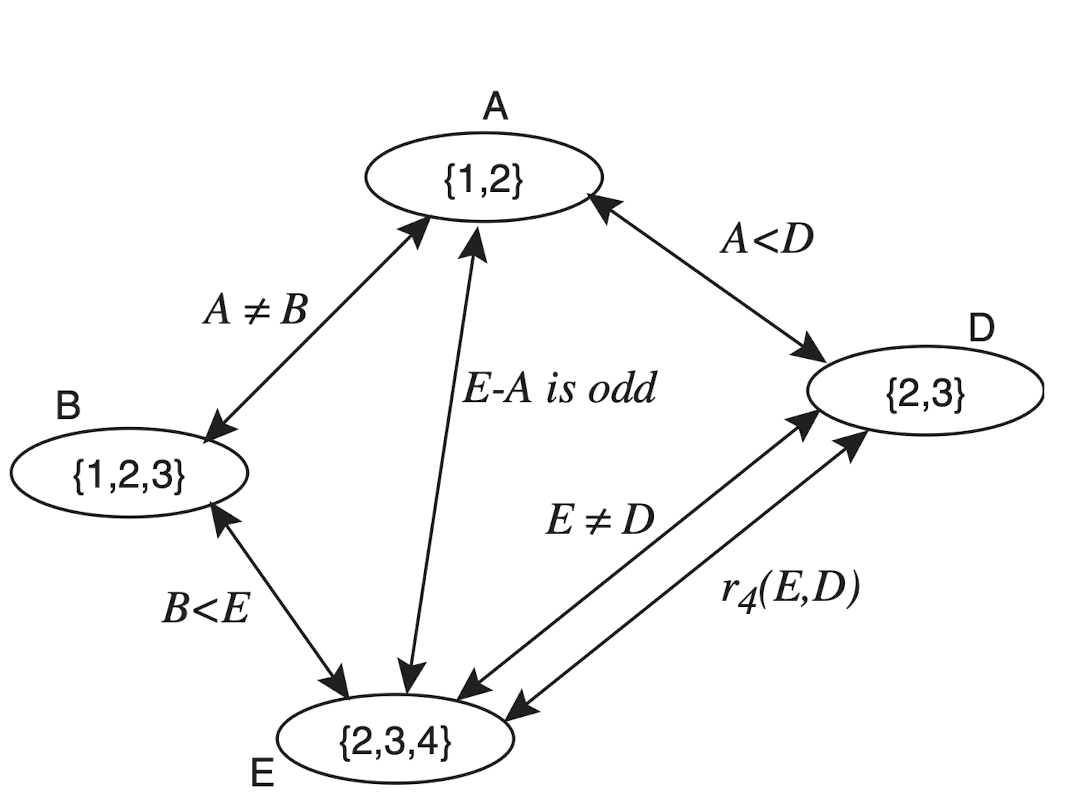
\includegraphics[width=5cm]{Variable_Elimination_2.png}
  	\end{figure*}
 \end{itemize}
  	

  \item \textbf{Local Search:} (Back to CSP as Search)
  \begin{itemize}
    \item Maintain a variable assignment, select neighbors to improve heuristic value, and stop when a satisfying assignment is found, or return the best assignment found.
    \item Aim is to find an assignment with zero \textbf{unsatisfied constraints (Conflict)}
    \item Goal is an assignment with \textbf{zero conflicts} (heuristic: \# of conflicts)
  \end{itemize}

  \item \textbf{Greedy Descent Variants:}
  \begin{itemize}
    \item At every step:\\
     (Select the variable-value pair that \textbf{minimize} \# of conflicts)\\
    (Select a variable involved in the \textbf{most} \# of conflicts, then a value \textbf{minimize} \# of conflicts)\\
    (Select a variable involved in \textbf{any} conflicts, then a value \textbf{minimize} \# of conflicts)
    
    (Select a variable \textbf{at random}, then a value \textbf{minimize} \# of conflicts)\\
    (Select a variable and value \textbf{at random}, accept if \textbf{doesn't increase}\footnote{Sometime accept even increase \# of conflicts to escape local minimum} \# of conflicts)
   
  \end{itemize}
  \newpage
  \item \textbf{GSAT (Greedy SATisfiability):}
 
 \begin{minipage}{.85\linewidth}
  \begin{itemize}
    \item Start with a random assignment of values to all variables $n$ \\heuristic $h(n)$ = \# of unsatisfied constraints 
    \item repeat until heuristic becomes 0 (Solved):
    \subitem Evaluate neighbours of n (not $n$, cannot change same variable twice in a row);
    \subitem Let $n$ be  the neighbour $n'$ that minimizes the heuristic, even if $h(n') > h(n)$.
    \item \textbf{Problems:}
   	\subitem stuck at local minimum, cannot pass a \textbf{plateau} where $h(n)$ are uninformative.
   	\subitem \textbf{Ridge} is a local minimum where \textbf{n-step look-ahead} might help.
   	\item \textbf{Randomized GSAT}: allow move to a random neighbour, reassign all variable randomly.
   	\end{itemize}
 \end{minipage}
  \hfill
  \begin{minipage}{.3\linewidth}
  	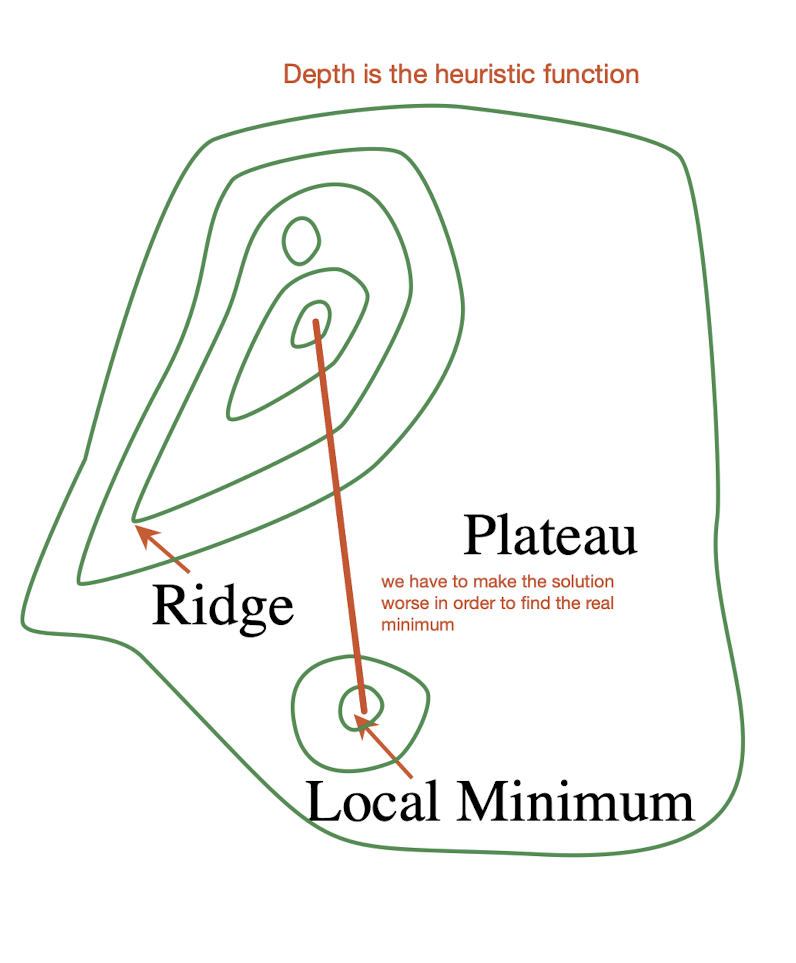
\includegraphics[width=.9\linewidth]{GSAT.png}
  \end{minipage}
   	
   	\begin{itemize}
   		\item \textbf{Tabu lists}: 
   		\subitem Maintain a tabu list of $k$ last assignments to prevent cycling.
   		\subitem Reject assignments exist on tabu lists.\footnote{e.g: $k=1$ means reject assignment of the same value to the variable chosen.}
   		\subitem More efficient than a list of complete assignments, but expensive if $k$ is large.
   	\end{itemize}
   	\item \textbf{Stochastic local search} is a mix of: 
   	
   		\begin{minipage}{.59\linewidth}
   			\begin{itemize}
   	\item \textbf{Greedy descent}: Move to a lowest neighbour (GSAT)
   	\item \textbf{Random walk}: taking some random steps
   	\item \textbf{Random restart}: reassigning all values randomly
   	\end{itemize}
   		\end{minipage}
   		\hfill
   		\begin{minipage}{.5\linewidth}
  	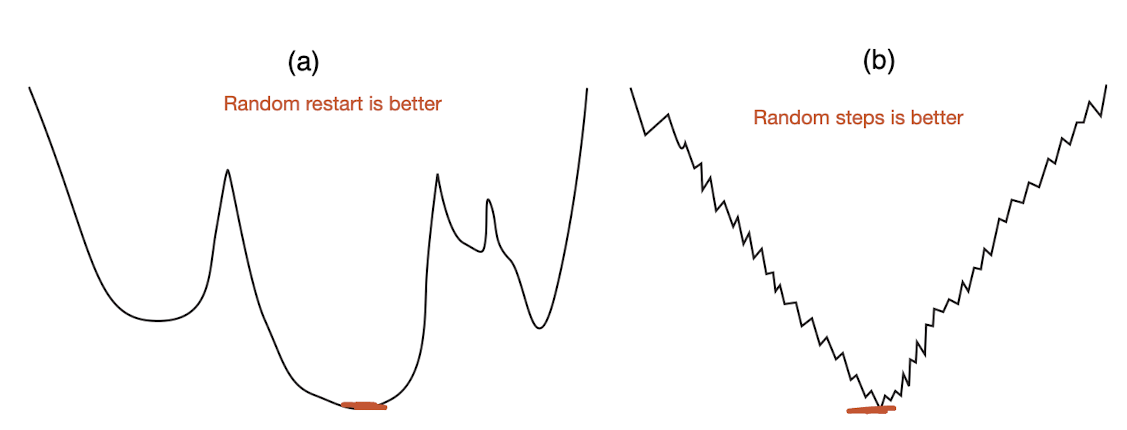
\includegraphics[width=\linewidth, height=2cm]{RGSAT.png}
   		\end{minipage}
   	
   	
   	\item \textbf{Simulated Annealing} (Variant of Stochastic local research)
   	\begin{itemize}
   		\item Pick a random value for a random variable (neighbour):
   		\subitem  Adopt if its an improvement.
   		\subitem  If it's not an improvement, adopt it probabilistically based on temperature $T$. (High $\rightarrow$ Low)
   		\subitem (move from current assignment $n$ to new assignment $n'$ with probability $e^{-\frac{h(n')-h(n)}{T}}$)\footnote{difference in heuristic value divided by temperature}
   		\subitem Terminate when criteria is met.
   	\end{itemize}
   	
   	\item \textbf{Parallel Search:}
  \begin{itemize}
    \item Maintains a population of \( k \) individuals (total assignments).
    \item Updates each individual in the population at every stage.
    \item Reports when any individual is a solution.
    \item Operates like \( k \) restarts but with \( k \) times the minimum steps.
  \end{itemize}

  \item \textbf{Beam Search:}
  \begin{itemize}
    \item Similar to parallel search with \( k \) individuals, but \textbf{choosing the \( k \) best from all neighbours}.
    \subitem (All if there are less than $k$)
    \item Reduces to greedy descent when \( k = 1 \).
    \item The value of \( k \) limits space and facilitates parallelism.
  \end{itemize}

  \newpage
  \item \textbf{Stochastic Beam Search:}
  \begin{itemize}
    \item A probabilistic variant of beam search, choosing \( k \) individuals for the next generation.
    \subitem (probability of a neighbour $n$ is chosen is proportional to $e^{-\frac{h(n)}{T}}$)
    \item Maintains diversity among individuals and reflects their fitness (heuristic).
    \item Operates like asexual reproduction, with mutation allowing fittest individuals to prevail.
  \end{itemize}

  \item \textbf{Genetic Algorithms:}
  \begin{itemize}
    \item  Like stochastic beam search but \textbf{combines pairs of individuals to create offspring}.
    \item Fittest individuals are more likely to be chosen for reproduction.
    \item Crossover and mutation (change some value) to form new solutions.
    \item Continues until a solution is found.
  \end{itemize}

  \item \textbf{Crossover:}
  \begin{itemize}
    \item Given two individuals, each offspring's attributes are randomly chosen from one of the parents.
    \item The effectiveness depends on the ordering of variables, many variations are possible.
  \end{itemize}

  \item \textbf{Comparing Stochastic Algorithms:}
  \begin{itemize}
    \item Considers how to compare algorithms with different success rates and runtimes.
    \item Acknowledges that summary statistics like mean, median, or mode runtimes may not be informative.
  \end{itemize}

  \item \textbf{Runtime Distribution:}
  \begin{itemize}
    \item Plots runtime or steps against the proportion of runs solved within that time.
    \item Helps in understanding the performance distribution of stochastic algorithms.
  \end{itemize}
   	
  \end{itemize}
  
  \section{Inference and Planning}
  	
  \begin{itemize}
  	\item 
  \end{itemize}
  


 














\end{document}
